\documentclass[12pt,addpoints]{exam}		%Doc : https://mirrors.ircam.fr/pub/CTAN/macros/latex/contrib/exam/examdoc.pdf
%   \printanswers					%Comment this line to hide the answers 
\usepackage[utf8]{inputenc}
\usepackage[T1]{fontenc}
\usepackage[english]{babel}      %Originally for french document, change to english or relevant language
\usepackage{amsmath,amssymb}
\usepackage{multicol}
\usepackage[dvipsnames]{xcolor}
\usepackage{tikz}
	\usetikzlibrary{fadings}
	\usetikzlibrary{calc}
\usepackage{tkz-tab}
\usepackage{pgfplots,float}
\usepackage{polynom}
\usepackage{hyperref}
\hypersetup{
      breaklinks=true,  % so long urls are correctly broken across lines
      colorlinks=true,
      urlcolor=urlcolor,
      linkcolor=linkcolor,
      citecolor=citecolor,
      }
    % Colors for the hyperref package
    \definecolor{urlcolor}{rgb}{0,.145,.698}
    \definecolor{linkcolor}{rgb}{.71,0.21,0.01}
    \definecolor{citecolor}{rgb}{.12,.54,.11}

\newcommand {\res}[1]{\resizebox{1\linewidth}{!}{$#1$}}
\polyset{%
  style=D}
%Format Header and footer
\pagestyle{headandfoot}
\header{\footnotesize Year: 2022/2023}{\Large\textbf{Higher National School of Mathematics\\}}{\footnotesize Mathematical Computing Tools}
\headrule
\usepackage{geometry}
 \geometry{
 a4paper,
 top=25mm,
 right=25mm,
 left=25mm,
 bottom=25mm
 }

 \footrule
\setlength{\columnsep}{0.25cm}
%\setlength{\columnseprule}{1pt}
%  \footer{   \begin{tabular}{c p{2.6cm}}
%     LastName: & \hrule \\ 
%        \end{tabular}}{\begin{tabular}{c p{2.6cm}}
%     FirstName: &\hrule  \\
%    \end{tabular}}{\begin{tabular}{c p{2.6cm}}
%     Group:& \hrule \\
%    \end{tabular}
%    }
%\extrafootheight{-2cm}

% Change section command behaviour
\usepackage{titlesec,cancel}
\usepackage[normalem]{ulem} 
\titleformat{\section}[frame]{\bfseries\filright}{}{2mm}{\centering List Of Projects \\ (Classical cryptography)}

% Add a watermark if answers are shown
% \ifprintanswers
% \usepackage{draftwatermark}
% \SetWatermarkColor{red!30}
% \SetWatermarkScale{5}
% % \SetWatermarkText{Draft}     %Watermark text
% \fi

%Format the name of each exercise
% \qformat{\textbf{Project \thequestion~(\thepoints):}\hfill}
 \qformat{\textbf{Project \thequestion~}\hfill}
\extrawidth{1cm}
\renewcommand\partlabel{\arabic{partno}.\ }
\newcommand{\red}[1]{\textcolor{red}{#1}}
\newcommand{\K}[1]{\mathbb{#1}}
\newcommand{\C}{\mathbb{C}}
\newcommand{\R}{\mathbb{R}}
\newcommand{\Q}{\mathbb{Q}}
\newcommand{\Z}{\mathbb{Z}}
\newcommand{\N}{\mathbb{N}}
\renewcommand\partlabel{\arabic{partno}.}
\renewcommand{\thesubpart}{(\alph{subpart}) }
\renewcommand{\subpartlabel}{\thesubpart}

%
% \title{Title}
\begin{document}

\section{}
\subsection*{Team Projects}
\begin{questions}

\question
{\center \bf Sliding Image Puzzle\\}
You have been assigned to develop a program that will aid a {\bf sliding
image puzzle} manufacturer in partitioning images for their puzzles.

\begin{figure}[H]
\centering
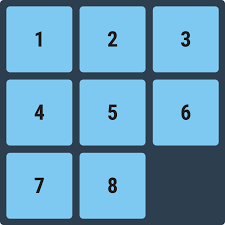
\includegraphics[scale=.5]{sliding_puzzle.png}
\caption{Sliding Puzzle}
\end{figure}

The program should be designed to accomplish the following tasks:

\begin{itemize}
\item \textbf{Task 1} Read \verb|images.txt|, which contains the links to the images.
 \begin{figure}[H]
  \centering
  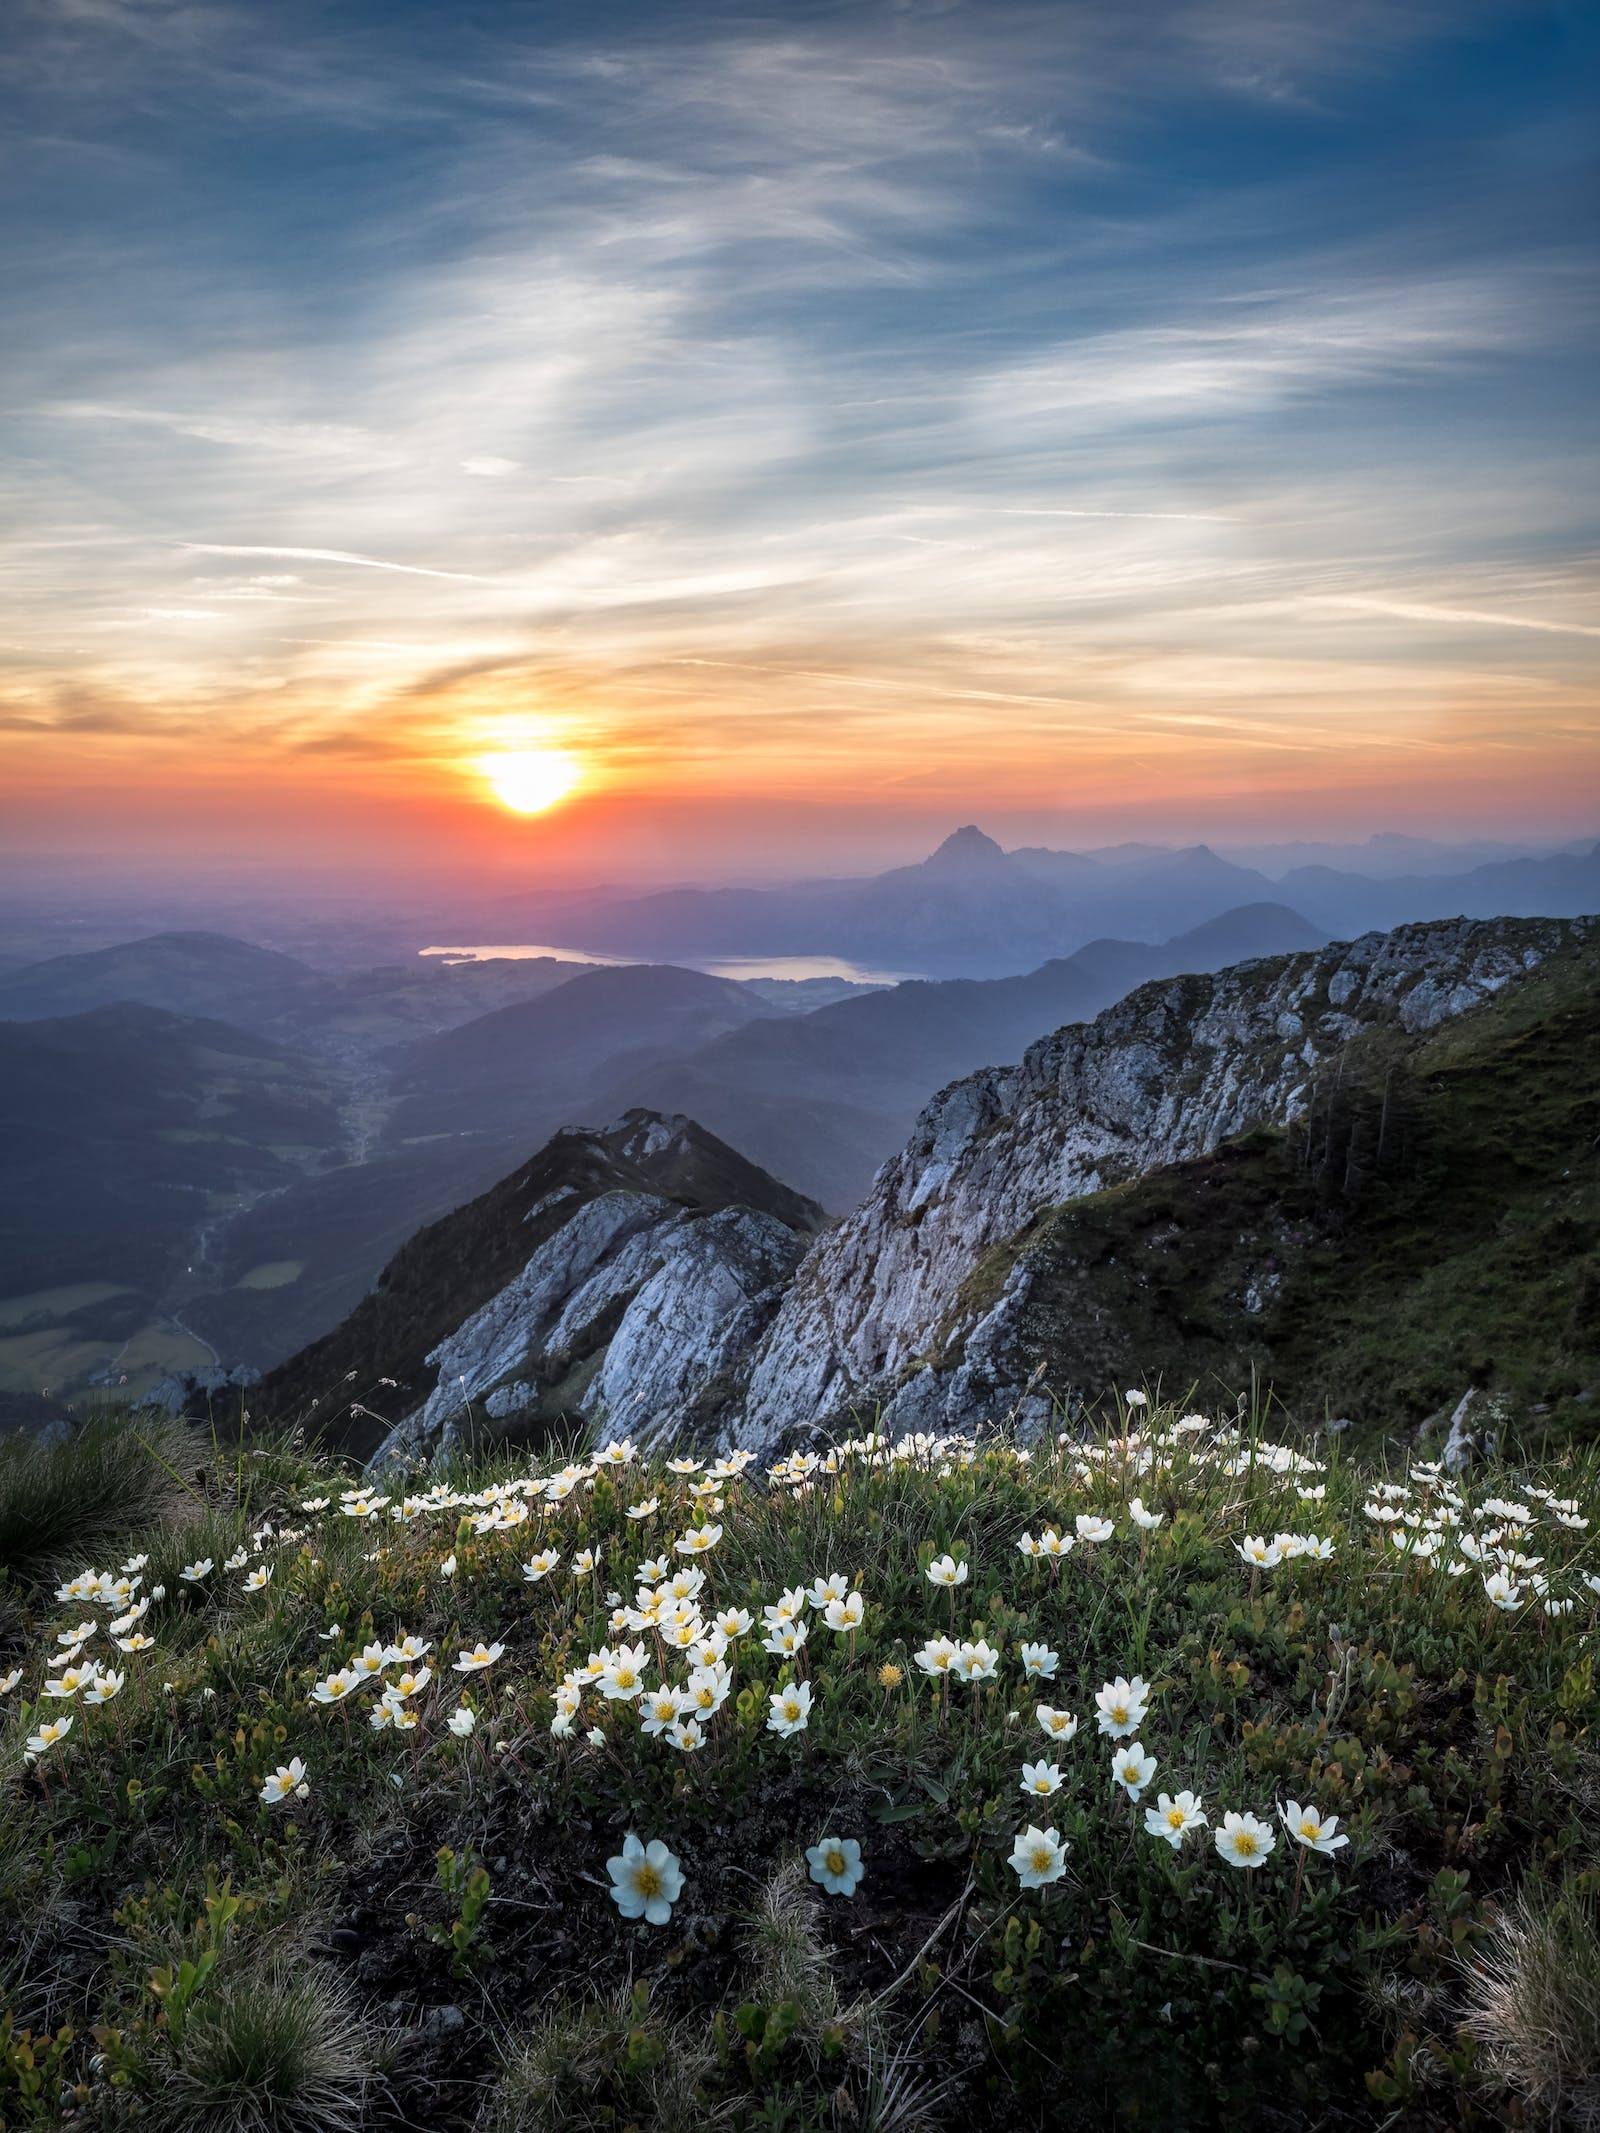
\includegraphics[scale=.088]{nature.jpeg}
  \end{figure}
  \href{https://ydjemmada.github.io/projects/images.txt}{Click here to get images.txt}
\item \textbf{Task 2} For images that are not square-shaped, crop them to obtain the maximum-sized square image possible located in the middle of the original image.
\begin{figure}[H]
\centering
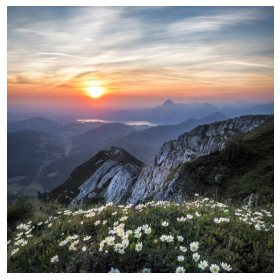
\includegraphics[scale=.5]{image_croped.png}
\end{figure}

\item \textbf{Task 3} Partition each image into eight equal parts, as
  illustrated in the the follwing figure.

\begin{figure}[H]
\centering
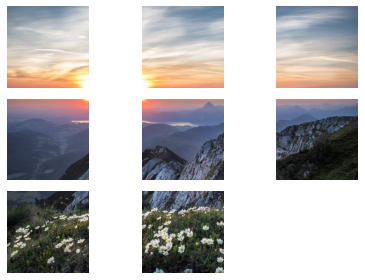
\includegraphics[scale=.5]{image_order.png}
\end{figure}


\item \textbf{Task 4} Generate a permuted grid of the eight small parts of the cropped image.

\begin{figure}[H]
\centering
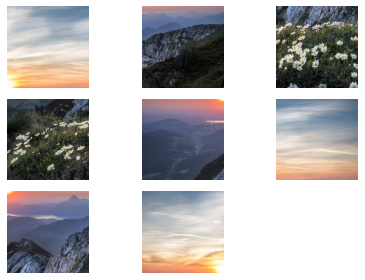
\includegraphics[scale=.5]{image_slides.png}
\end{figure}

\item \textbf{Task 5} Store each cropped image and its corresponding eight small parts in a directory named \verb|puzzle_i|, where \verb|i| represents the image's order in the file.
\end{itemize}

Your program should be programmed to perform these tasks effectively and
efficiently. It should be thoroughly documented, and clear instructions
should be provided to your users.
\newpage
\question
{\center \bf Medical Image Encryption and Decryption using XOR and PRNGs\\}

A clinic has to send medical images to another institution, but they are
concerned about the safety of the images in transit. They have requested
your help to develop a solution to secure the images so that they cannot
be intercepted or accessed by unauthorized individuals.

\hypertarget{project-requirements}{%
\paragraph{Project Requirements}\label{project-requirements}}

Your task is to create a program that will encrypt the medical images
using XOR and pseudo-random number generator (PRNG) and then save the encrypted images to a safe
location. You will then decrypt the encrypted images using the same
function to ensure that the original images are restored.

To achieve this, you will need to complete the following steps:

\begin{itemize}
\item
  \textbf{Task 1} Read the list of medical images from the given directory. \href{https://ydjemmada.github.io/projects/proj2_images.rar}{Download the set of images from here}
  \begin{figure}[H]
    \centering
    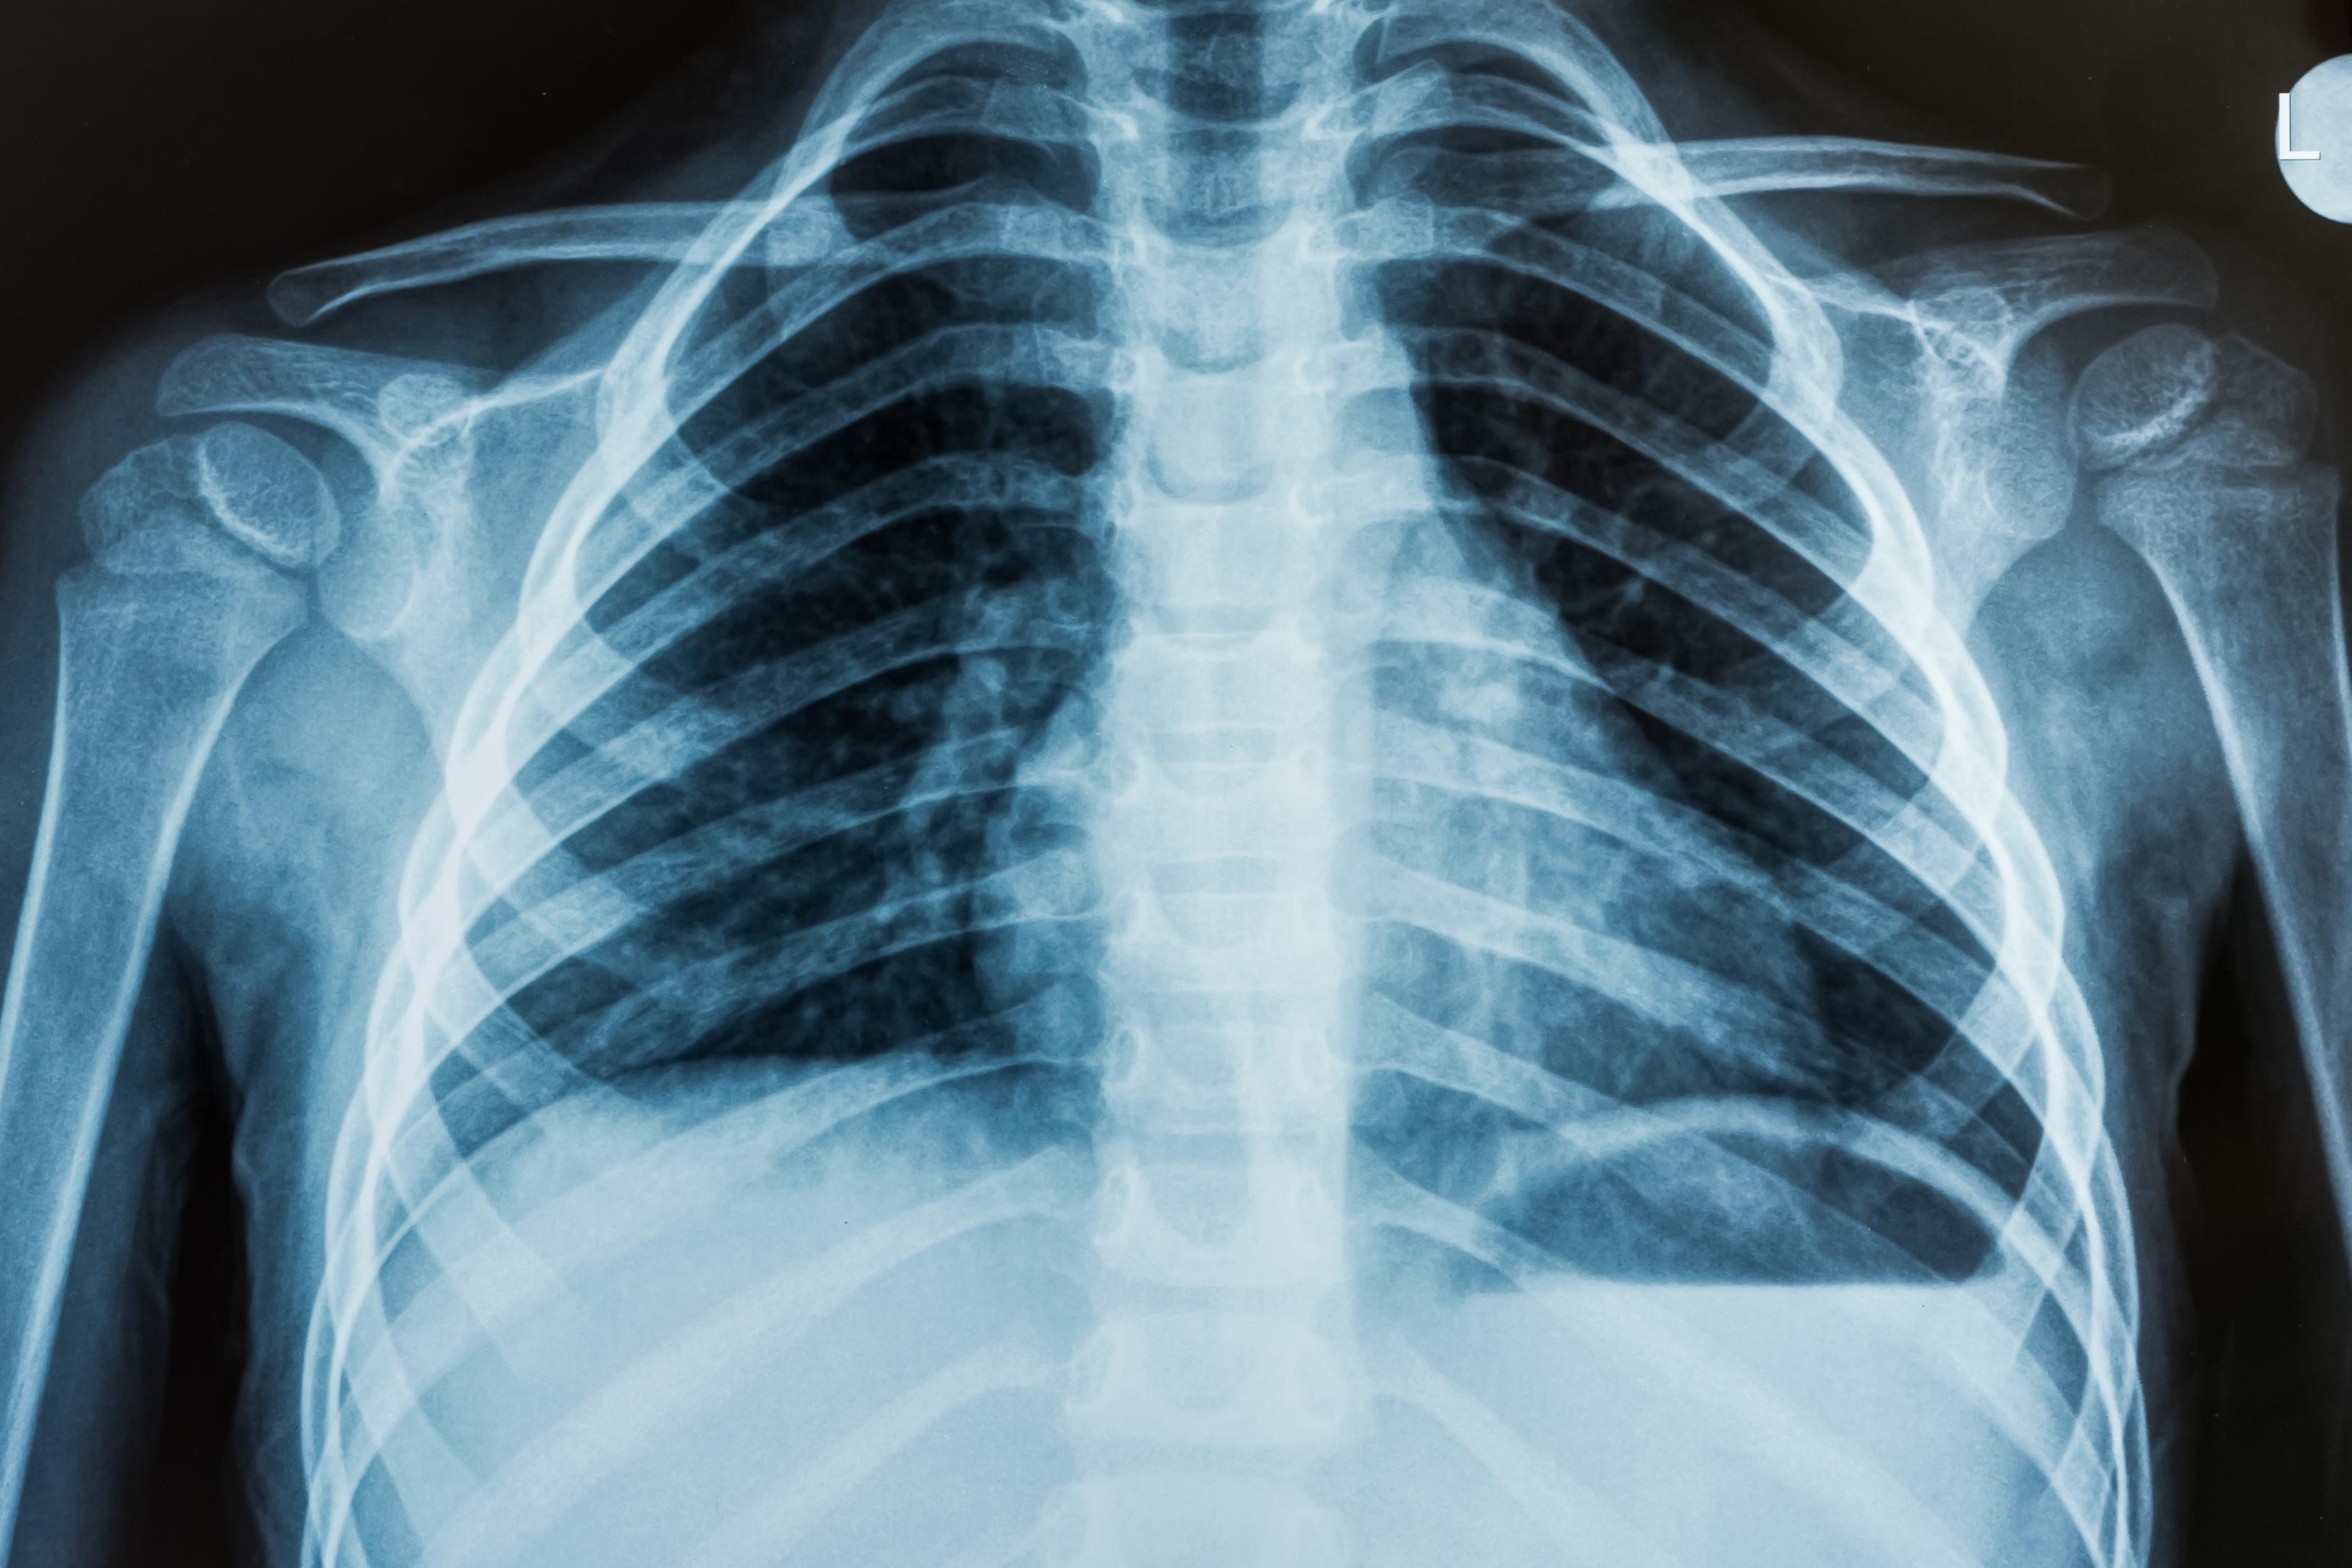
\includegraphics[width=150px]{med_1.jpg} 
  \end{figure}
  \item
  \textbf{Task 2} Implement with python three PRNGs using any of the PRNG algorithms
  available (e.g., Lehmer generator).
  \href{https://en.wikipedia.org/wiki/List_of_random_number_generators}{List
  of prngs}
\item
  \textbf{Task 3} For each medical image, encrypt the image using XOR with a list of random numbers generated with the three PRNGs: xor each byte with a byte from the prng output.
  \begin{figure}[H]\centering
    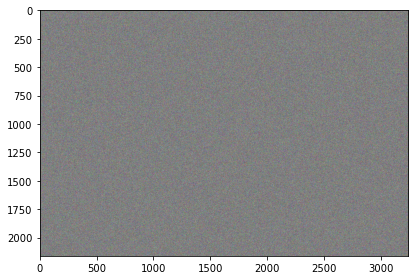
\includegraphics[width=200px]{enc_med_1.png} 
  \end{figure}
\item
  \textbf{Task 4} Save the encrypted image in a folder named \verb|encrypted_data|.
\item
  \textbf{Task 5} For each encrypted image, decrypt the image using the same XOR function and PRNGs (use the same keys as encryption step).
\item
  \textbf{Task 6} Compare the decrypted image with the original image to ensure that the image was decrypted successfully.
\item
  \textbf{Task 7} Write a report on the project, including details on the implementation, the results, and any challenges encountered.
\end{itemize}
\newpage
\question
{\center \bf The $0\text{-}1$ Knapsack problem\\}
The $0\text{-}1$ Knapsack problem is a classic optimization problem in computer
science and mathematics. The problem is defined as follows:

Given a set of items, each with a weight and a value, and a knapsack
with a maximum weight capacity, determine the maximum value that can be
put into the knapsack without exceeding its weight capacity.

In the $0\text{-}1$ version of the problem, each item can only be taken once
(either included in the knapsack or not), hence the name ($0\text{-}1$). The
goal is to maximize the total value of the items in the knapsack while
keeping the weight of the knapsack within the maximum capacity.

The $0\text{-}1$ Knapsack problem has important applications in various fields,
such as resource allocation, financial portfolio optimization, and
logistics planning.

\begin{itemize}
\item
  \textbf{Task 1}: Problem Description Write a brief description of the
  $0\text{-}1$ Knapsack problem, including its goal, and how it can be
  represented as a graph.
\item
  \textbf{Task 2}: Research the dynamic programming Method Research the
  dynamic programming Method and write a brief explanation of how it
  works, including the steps involved in solving the $0\text{-}1$ Knapsack
  problem.
\item
  \textbf{Task 3}: Implement the dynamic programming method Implement
  the dynamic programming in Python, using NumPy to perform the
  necessary calculations.
\item
  \textbf{Task 4}: Test the Implementation Test the implementation using
  a small example problem and verify that it produces the correct
  solution.
\item
  \textbf{Task 5}: Write a Report Write a report summarizing the
  project, including the problem description, the solution approach, the
  implementation details, and the test results.
\end{itemize}

\textbf{References}:

\begin{enumerate}
\def\labelenumi{\arabic{enumi}.}
\item
\href{https://en.wikipedia.org/wiki/Knapsack\_problem}{https://en.wikipedia.org/wiki/Knapsack\_problem}
\end{enumerate}
\newpage
\question
{\center \bf COVID-19 Detector\\}
A hospital has reached out to us for help in classifying a large dataset of X-ray images to determine whether a person has COVID-19 or not. The hospital has been overwhelmed with patients and needs an automated system to assist their medical staff in diagnosing COVID-19 accurately and efficiently.


The project will consist of the following tasks:


\begin{itemize}
    \item
      \textbf{Task 1}: Read the gray images in the data set image by image, \href{https://ydjemmada.github.io/projects/xrays.zip}{Download the data set from here}.
    \item
      \textbf{Task 2}: Calculate the average of pixels having a value $\geq 128$ (near to white color) for each image
    \item
      \textbf{Task 3}: Classify the image based on the calculated average
      value:
    
      \begin{itemize}

      \item
        if the average $\leq 50$, the person is negative for Covid
      \item
        if the average $>50$ and $\leq 60$, the person is
        suspected to have Covid
      \item
        if the average $>60$, the person has Covid
      \end{itemize}
    \item
      \textbf{Task 4}: Process the images depending on their Covid status:
    
      \begin{itemize}

      \item
        Convert the gray images to RGB format
      \item
        For negative Covid images, add a green border to the image
      \item
        For suspected Covid images, add an orange border to the image
      \item
        For confirmed Covid images:
    
        \begin{itemize}

        \item
          Split the image vertically into two parts
        \item
          Calculate the average pixel value near to white for each part
        \item
          Determine which part of the image has a higher average value
        \item
          Add a red border to the original image on the side of the sick
          lung
        \end{itemize}
      \end{itemize}
    \item
      \textbf{Task 5}: Save the final result image to a folder named \verb|results|
    \end{itemize}
\begin{center}
        \begin{minipage}{.27\linewidth}
            \begin{figure}[H]
                \centering
                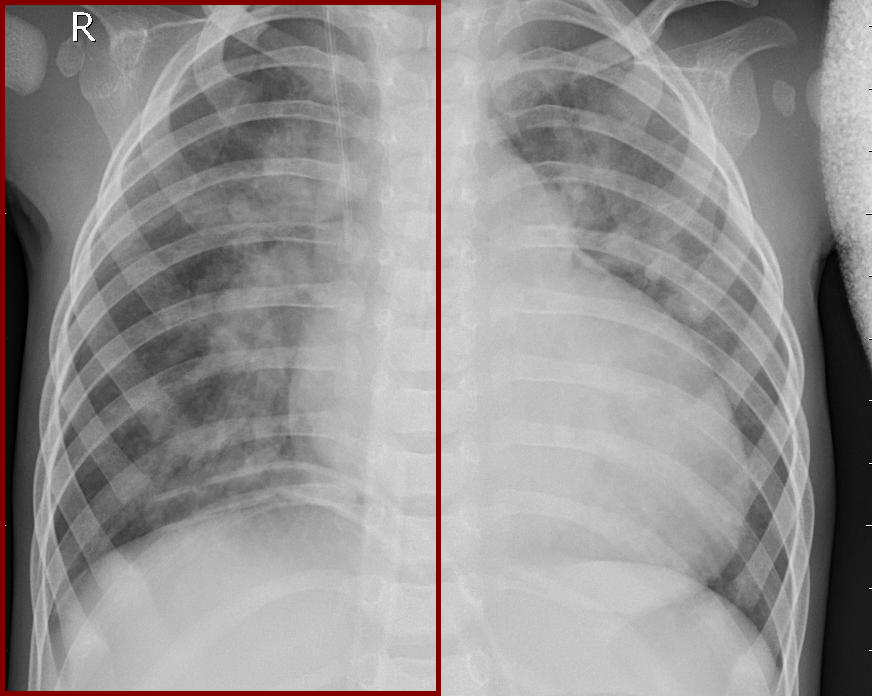
\includegraphics[width=110px]{red_border.png}
            \end{figure}
        \end{minipage}
        \begin{minipage}{.27\linewidth}
            \begin{figure}[H]
                \centering
                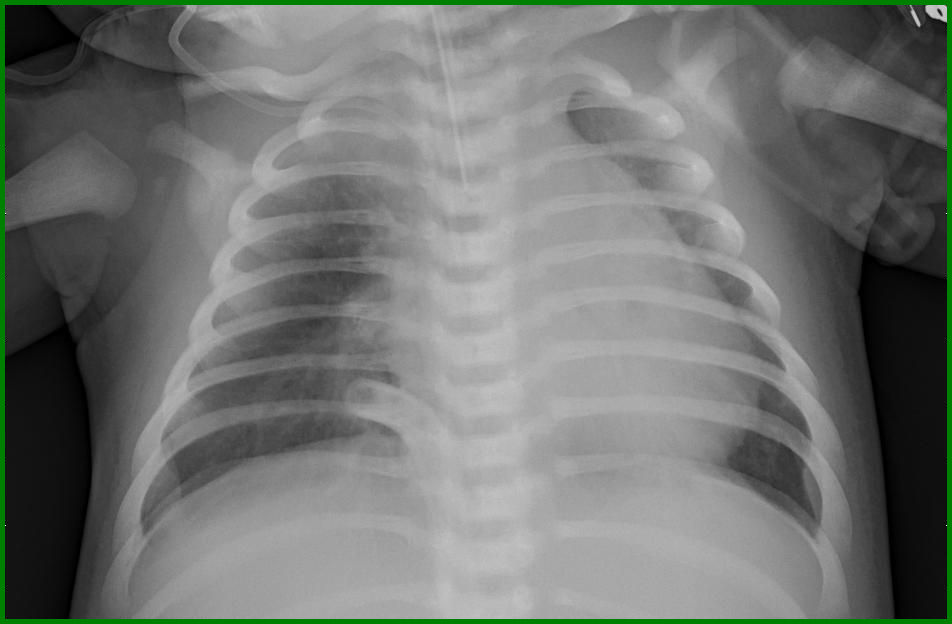
\includegraphics[width=110px]{green_border.png}
            \end{figure}
        \end{minipage}
        \begin{minipage}{.27\linewidth}
            \begin{figure}[H]
            \centering
                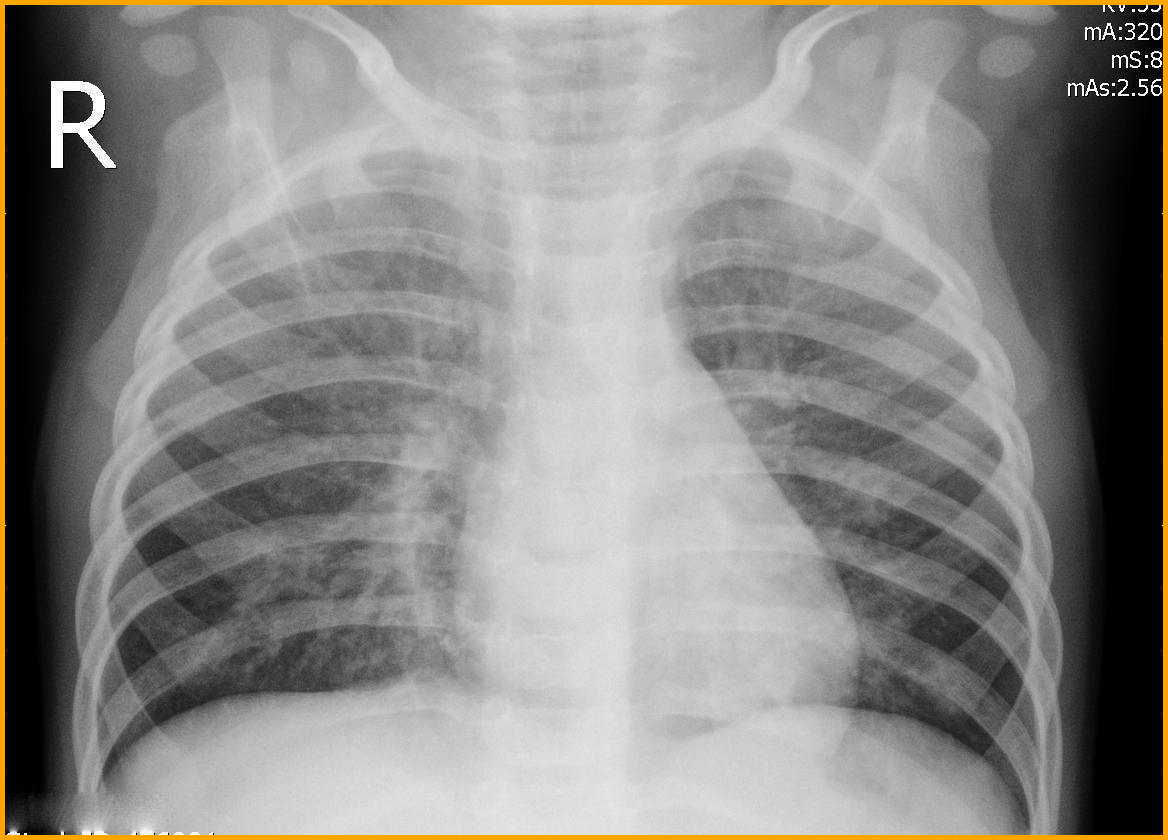
\includegraphics[width=110px]{orange_border.png}
            \end{figure}
        \end{minipage}
\end{center}

                  
    
    You can further break down each task into subtasks and write code to
    accomplish each subtask.
\newpage
\question
{\center \bf Solving the Assignment Problem using the Hungarian Method\\}
The assignment problem is a classic optimization problem in which a set
of agents must be assigned to a set of tasks, with each agent being
assigned to exactly one task and each task being assigned to exactly one
agent. The goal is to minimize the total cost or time required for the
assignments, which can be represented as a square cost matrix, where the
element in row i and column j represents the cost of assigning agent i
to task j.

\begin{itemize}
\item
  \textbf{Task 1}: Problem Description Write a brief description of the
  Assignment Problem, including its goal, and how it can be represented
  as a square cost matrix.
\item
  \textbf{Task 2}: Research the Hungarian Method Research the Hungarian
  Method and write a brief explanation of how it works, including the
  steps involved in solving the Assignment Problem.
\item
  \textbf{Task 3}: Implement the Hungarian Method Implement the
  Hungarian Method in Python, using NumPy to represent the cost matrix
  and perform the necessary calculations.
\item
  \textbf{Task 4}: Test the Implementation Test the implementation using
  a small example problem and verify that it produces the correct
  solution.
\item
  \textbf{Task 5}: Write a Report Write a report summarizing the
  project, including the problem description, the solution approach
  using the Hungarian Method, the implementation details, and the test
  results.
\end{itemize}

\textbf{References}:

\begin{enumerate}

\item
  \href{http://biblio.univ-antananarivo.mg/pdfs/randrianatoandroFenoarisoaT\_MP\_MAST\_21.pdf}{http://biblio.univ-antananarivo.mg/pdfs/randrianatoandroFenoarisoaT\\\_MP\_MAST\_21.pdf}
\item
  \href{https://en.wikipedia.org/wiki/Hungarian\_algorithm}{https://en.wikipedia.org/wiki/Hungarian\_algorithm}
\end{enumerate}

\question
{\center \bf Random generators' tests\\}
\href{https://ydjemmada.github.io/projects/Project\_6.pdf}{Find the project details here: https://ydjemmada.github.io/projects/Project\_6.pdf}
\question
{\center \bf Will be here soon\\}
%+project 7
\end{questions}
\subsection*{Individual Projects}
You should choose one of the project: 
\begin{itemize}
  \item \textbf{RSA encryption scheme},
  \item \textbf{3DES encryption scheme}, 
  \item \textbf{EL-GAMAL encryption scheme}, 
  \item \textbf{Diffie--Hellman key exchange.}
\end{itemize}

or 4 project of the 6th teams' project or join a team.
\end{document}